\chapter{A Rust futtatókörnyezet, útvonalkeresés és vizualizáció}

A korai szakaszban elegendő volt egy könnyebb, főleg frontend-demóra épülő útvonalkereső prototípus. Ahogy azonban a háló, a felület és az analitikai ambíciók nőttek, egyre nyilvánvalóbbá vált, hogy a futásidejű gráfmodellnek külön, stabilabb végrehajtási környezetre van szüksége. A Rust bevezetése nagyobb teljesítményt, kiszámíthatóbb memóriakezelést, determinisztikusabb gráfállapotot és tisztább határt ad a böngésző és a számítás között.

\section{A Rust gráfállapot}

A Rust réteg a gráfot közvetlenül a meccs-JSON állományokból és a játékos-adatbázisból építi fel, és két nézetet hoz létre: a \textit{population graph} globális, súlyozott együtt-játszási nézet; a \textit{pathfinder graph} olyan futásidejű modell, amely külön tárolja az \textit{allyWeight}, \textit{enemyWeight} és \textit{totalMatches} értékeket. Ez az a pont, ahol a rendszer átmegy egyszerű együtt-játszási hálóból olyan gráffá, amelyen már nemcsak közösségeket, hanem előjeles kapcsolatokat és többféle útvonalmódot is lehet vizsgálni.

A \textit{GraphState} a szomszédsági listák mellett tárolja a \textit{pair\_relations} szerkezetet, a játékosprofilok gyors elérését, a klasztertagságot, a klaszter-összegzéseket, a landmark-távolságokat, a minimumköltségeket és az aktív datasethez tartozó snapshot-metaadatot. A runtime nem pusztán kereséshez optimalizált gráf, hanem a kutatási analitikák és az exportok közös memóriabeli alapja.

A \textit{build\_graph\_state()} felépítési sorrendje önmagában is fontos architektúrális állítás: a motor előbb feloldja az aktív dataset útvonalait, betölti a játékosprofilokat, felépíti az élstruktúrát, létrehozza vagy frissíti a Rust oldali klasztereket, majd ezután készíti elő a gyorsító struktúrákat (landmark- és minimumköltség-táblákat). A teljesítményoptimalizálás tehát nem üres, steril gráf fölött történik, hanem egy már szemantikailag gazdag állapoton.

\diagramfigure{A Rust Pathfinder keresési tevékenységdiagramja - a négy algoritmus döntési pontjai és visszaterjesztési lépései}{rust pathfinder activity diagram.pdf}

\section{Útvonalkereső algoritmusok}

A jelenlegi Rust futtatókörnyezet négy algoritmust támogat: BFS, Dijkstra, kétirányú keresés és A*. Az algoritmusok két különböző élértelmezésben futhatnak: \textit{social-path} csak szövetségesi kapcsolatokon, \textit{battle-path} összes ismétlődő kapcsolaton. Súlyozott módban az erősebb, többször ismétlődő kapcsolatok olcsóbb élköltséget kapnak, ami azt fejezi ki, hogy az erősebb ismétlődő viszonyok „közelebb vannak" egymáshoz a gráfban.

Az élköltség-modell egyszerű és magyarázható. Súlyozatlan módban minden él költsége fix $1000$. Súlyozott módban:

\begin{equation}
c(u,v)=\left\lceil \frac{1000}{w(u,v)} \right\rceil
\end{equation}

ahol $w(u,v)$ az adott útvonalmódnak megfelelő kapcsolaterősség (\textit{social-path} módban az \textit{allyWeight}, \textit{battle-path} módban a \textit{totalMatches}). Az $1000$-es egész skála determinisztikusabb sorrendezést biztosít az egész értékű prioritásos soroknál.

\begin{table}[H]
\centering
\caption{A Pathfinder Labban szereplő algoritmusok összevetése}
\begin{tabularx}{\textwidth}{>{\raggedright\arraybackslash}p{2.8cm} >{\raggedright\arraybackslash}p{2.8cm} X}
\toprule
\textbf{Algoritmus} & \textbf{Mikor természetes?} & \textbf{Megjegyzés a projektben} \\
\midrule
BFS & súlyozatlan legrövidebb út & Jó baseline, könnyen magyarázható \\
Dijkstra & súlyozott utak & Referenciaalgoritmus a költség-alapú módokban \\
Kétirányú keresés & nagyobb gráf, kevésbé irányított keresés & Gyakorlati gyorsítás bizonyos esetekben \\
A* & jól kialakított alsó becsléssel & A projektben egzakt marad, nem csak vizuális heurisztika \\
\bottomrule
\end{tabularx}
\end{table}

\begin{figure}[h]
\centering
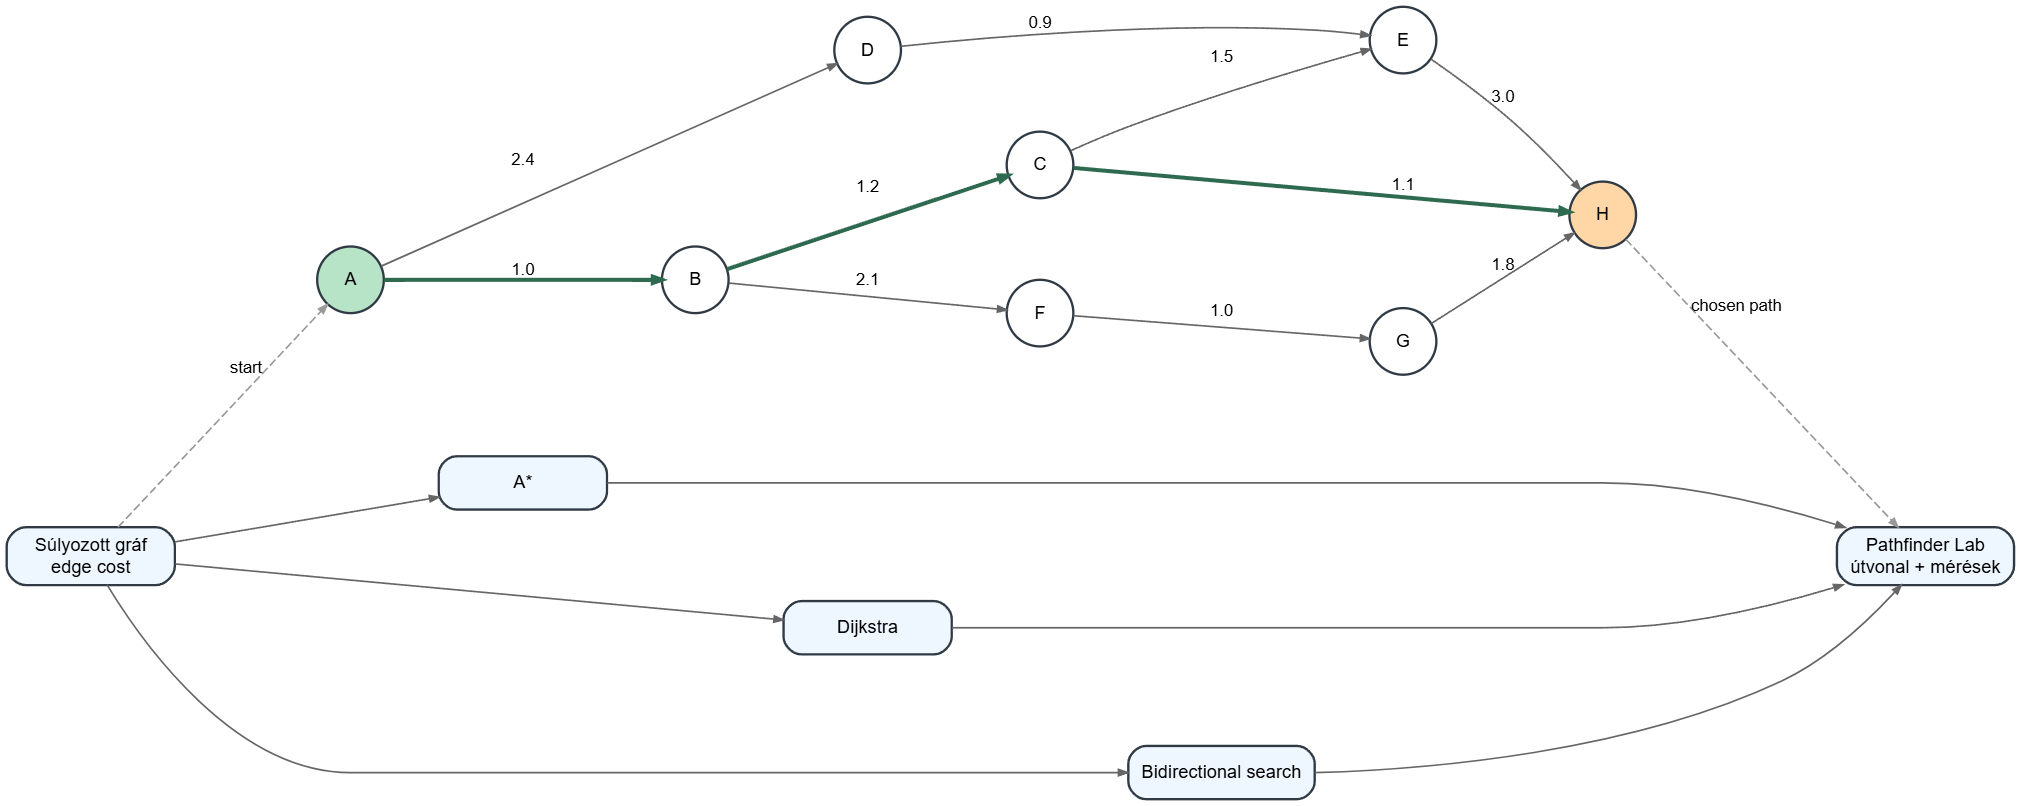
\includegraphics[width=0.92\textwidth]{assets/diagrams/thesis_pathfinding_graphviz.png}
\caption{A Pathfinder Lab algoritmikus értelmezése: ugyanazon súlyozott gráfon több keresési stratégia futtatható, majd az eredmény a replay és mérési rétegen keresztül válik összehasonlíthatóvá.}
\label{fig:pathfinder-graphviz-overview}
\end{figure}

\diagramfigure{A Pathfinder Lab és a frontend komponensstruktúrája - a keresési kérelmek útja a React nézettől a Rust motorig}{path finder and frontend component diagram.pdf}

\subsection{Szélességi keresés (BFS)}

A BFS súlyozatlan módban garantáltan a minimális lépésszámú útvonalat adja. Az implementáció FIFO-sort (\textit{VecDeque}) tart fenn és leáll, amint a célcsomópont először felbukkan a szomszédsági listán. A trace-rögzítés jól mutatja, hogyan terjed ki a keresési határ egyenletesen minden irányban.

\diagramfigure{BFS futtatás a Pathfinder Labban - az egyenletes szélességi terjeszkedés és a minimális ugrásszámú útvonal jól látható a replay állapotban}{pathfinder-bfs-testrun.png}

\subsection{Dijkstra-algoritmus}

A Dijkstra-algoritmus \cite{dijkstra1959} bináris kupacot (\textit{BinaryHeap}) használ. A \textit{QueueState} struktúra lexikografikusan rendez: először az alacsonyabb \textit{cost}, másodlagosan az alacsonyabb csomópont-id szerint, ami garantálja, hogy azonos súlyú utak esetén determinisztikusan mindig ugyanazt az útvonalat kapjuk. Súlyozott módban a rendszer valóban a közvetett, de erős útvonalat preferálja a gyenge közvetlen éllel szemben.

\subsection{Kétirányú keresés}

A kétirányú BFS a forrásból és a célból párhuzamosan terjeszt ki egy-egy keresési frontot, és megáll, amint a két front találkozik. Az implementáció felváltva bővíti a forrás-oldali és a cél-oldali sort. Sűrű vagy nagy gráfokban a meglátogatott csomópontok száma közelítőleg $O(\sqrt{n})$ lehet az egyirányú $O(n)$-hez képest; a tényleges gyorsulás a klaszteres gráfon méréssel ellenőrizhető.

\subsection{A* keresés}

Az A* \cite{hart1968} a Dijkstra-algoritmust terjeszti ki célirányos heurisztikával. Az \textit{AStarState} a \textit{path\_cost} és a \textit{heuristic\_cost} összegével rendez. A heurisztika a \textit{GraphState}-ben előre kiszámított landmark-távolságok táblájából és \textit{cluster\_hops} adatból kombinál admisszibilis alsó becslést, így az A* helyes legrövidebb utat ad. Az egységtesztek igazolják, hogy az A* eredménye egyezik a Dijkstra-eredménnyel minden releváns esetben; csak a keresési sorrend más.

\section{Egzakt A* és heurisztika}

\subsection{Landmark-alapú ALT heurisztika}

Az ALT (A* + Landmarks + Triangle inequality) heurisztika \cite{goldberg2005} a következő elvből indul ki. Ha $L$ egy landmark-csomópont és $d(u, L)$ az $u$ csomópontból $L$-be vezető ismert távolság, akkor:

\begin{equation}
d(u, t) \geq |d(L, t) - d(L, u)| \quad \text{minden } L \text{ landmarkra}
\end{equation}

A rendszer az összes konfigurált landmarkra kiszámolja ezt a korlátot, és a maximumukat adja heurisztikaként. A landmark-távolságok a \textit{GraphState} felépítésekor előre kiszámítódnak minden \textit{ModeKey} kombinációra (SocialUnweighted, SocialWeighted, BattleUnweighted, BattleWeighted) Dijkstra-futtatással, és az összes keresési kérésre újrafelhasználhatók.

\subsection{Landmark-kiválasztás}

A \textit{choose\_landmarks()} a kiindulási landmark-halmazt prioritás alapján állítja össze: előbb hybrid cluster bridge-csomópontok (nagy valószínűséggel sok legrövidebb úton vannak), majd klaszterközéppontok, végül egyéb nagy fokszámú csomópontok. Ez garantálja, hogy a landmarkok a gráf szemantikailag fontos helyein legyenek, ahol a legjobb (legmagasabb) alsó becsléseket adják.

\subsection{Klaszterugrás-alapú becslés és tie-break}

A \textit{cluster\_hops} a forrás és cél klaszter közötti minimális klaszterugrásokon alapul, egy külön Dijkstra-futtatás eredménye a klaszter-szintű gráfon. Admisszibilis korlát, mert bármely útvonalnak legalább annyit kell haladni klasztereken keresztül, mint az inter-klaszter legrövidebb út. A tie-break a klaszterközpont-távolság alapján bont döntetlen azonos becsült összköltség esetén. A képernyőn látható közelség és a gráfbeli költség nem azonos fogalom; ha a rendszer a layoutot valódi heurisztikaként használná, az könnyen inadmisszibilissé tenné a keresést, ezt a megoldás tudatosan kerüli el.

\section{Pathfinder Lab}

A Pathfinder Lab az a réteg, ahol a Rust algoritmusok, a backend-szerződések, a perzisztens játékosprofilok és a böngészőben értelmezhető interakció egyetlen működő demonstrációvá állnak össze. A lab célja nem pusztán az, hogy két játékos között útvonalat megjelenítsen, hanem az, hogy algoritmusonként is láthatóvá tegye, mit jelent ugyanaz a keresési feladat eltérő számítási szemléletekkel megoldani.

A kimenetet a replay panel és a vizuális léptetés teszi értelmezhetővé. A motor minden releváns lépéshez képes rögzíteni az aktív csomópontot, a frontier rövidített állapotát, a meglátogatott csúcsok halmazát és a kiemelt éleket. Így a BFS, Dijkstra, kétirányú keresés és A* nem csak végső útvonal-hosszal hasonlítható össze, hanem a bejárási stratégia szintjén is. A magyarázhatóság nem utólagos vizuális díszítés, hanem a keresőmotor válaszformátumának része.

\diagramfigure{A Pathfinder Lab replay panele - az útvonalösszegző, a léptetési vezérlők és a meglátogatott csomópontok statisztikái}{pathfinder-replay-panel.png}

\diagramfigure{Az overlay vezérlőpanel - szünet, sebesség és vizualizációs beállítások a replay lejátszás közben}{pathfinder_replay_overlay.png}

Az alábbi mérési eredmény különösen szemléletes:

\begin{table}[H]
\centering
\caption{BFS és súlyozott keresés összehasonlítása - ugyanazon játékospár, eltérő közelségi fogalmak}
\begin{tabularx}{\textwidth}{>{\raggedright\arraybackslash}p{3cm} >{\raggedright\arraybackslash}p{3cm} >{\raggedright\arraybackslash}p{2cm} X}
\toprule
\textbf{Algoritmus} & \textbf{Metrika} & \textbf{Eredmény} & \textbf{Értelmezés} \\
\midrule
BFS & Minimális ugrásszám & 3 & Legrövidebb szociális lánc \\
Dijkstra & Min. súlyozott költség & 8 & Legerősebb szövetségesi útvonal \\
A* & Min. súlyozott költség & 8 & Egyezik Dijkstrával \\
Kétirányú & Min. ugrásszám & 3 & Egyezik BFS-sel \\
\bottomrule
\end{tabularx}
\end{table}

A BFS által talált 3-ugrás-os útvonal strukturálisan létezik, de gyenge vagy egyszeri meccsből eredő kapcsolatokon halad át. A Dijkstra súlyozott módban elkerüli ezeket, és helyette egy 8-ugrás-os útvonalat talál, amelyen minden él ismétlődő szövetségesi viszony. A két eredmény nem ellentmond egymásnak: két különböző közelségi fogalmat mér. Súlyozatlan módban a strukturális távolság a kérdés, a Milgram-féle ugrásos közelség értelmében \cite{milgram1967}; súlyozott módban a relációs gerinc kerül felszínre, melyik a legerősebb szövetségesi lánc. Granovetter \cite{granovetter1973} gyenge kapcsolatok elvének analógiájával: a gyenge kapcsolatok (BFS-útvonal) jobb információterjedési csatornák, az erős kapcsolatok (Dijkstra-út) határozzák meg a tényleges közösségi határokat. A BFS=3/Dijkstra=8 divergencia megmutatja, hogy a gráf látszólagos összefüggésének mekkora hányada valódi ismétlődő kapcsolatokból és mekkora alkalmi meccsfelállításokból ered.

\diagramfigure{A* keresés súlyozatlan módban - mindössze 60 csomópontot látogat meg a BFS 5906-ával szemben, mégis azonos 3-ugrás-os eredményt ad; a heurisztika egyenesen a célba irányítja a keresést}{pathfinder-astar-unweighted-testrun.png}

\diagramfigure{A* keresés súlyozott módban - a landmark heurisztika és a klaszter-alapú alsó becslés relációs erősség mentén irányítja a bejárást}{pathfinder-astar-weighted-testrun.png}

\diagramfigure{Az összes algoritmus futtatása súlyozatlan módban - BFS, Dijkstra, kétirányú és A* egységes összehasonlítása azonos játékospáron}{pathfinder-algocomparision-unweighted-test.png}

\diagramfigure{Az összes algoritmus futtatása súlyozott módban - Dijkstra és A* eltér a BFS és kétirányú keresés eredményétől; a heurisztikák csak súlyozott módban aktívak}{pathfinder-algocomparision-weighted-test.png}

\begin{table}[H]
\centering
\caption{A négy algoritmus összehasonlítása a legfontosabb dimenziók mentén}
\begin{tabularx}{\textwidth}{>{\raggedright\arraybackslash}p{3cm} >{\raggedright\arraybackslash}p{2.5cm} >{\raggedright\arraybackslash}X >{\raggedright\arraybackslash}X}
\toprule
\textbf{Algoritmus} & \textbf{Optimális?} & \textbf{Memória} & \textbf{Fő erősség a projektben} \\
\midrule
BFS & Igen (súlyozatlan) & $O(n)$ & Egyszerű baseline, jól magyarázható replay \\
Dijkstra & Igen (súlyozott) & $O(n + m)$ & Referencia-algoritmus, lexikografikus döntetlen-kezelés \\
Kétirányú & Igen (súlyozatlan) & $O(n)$ & Potenciális gyorsulás klaszteres gráfon \\
A* & Igen (heurisztika elfogadható) & $O(n)$ & Célirányos bejárás, egzakt eredmény \\
\bottomrule
\end{tabularx}
\end{table}

\section{Backend orchestráció}

A Rust analitikai parancsfolyam parancsvezérelt háttérfolyamat. A frontend HTTP/JSON kérést küld a Node.js backendnek, a backend a \textit{rustBridge.js} rétegen keresztül indítja vagy újrahasznosítja a Rust CLI folyamatot, és a tényleges parancs stdin csatornán JSON-ként jut el a Rust motorhoz, a válasz stdout-on érkező JSON objektumként kerül vissza. A Node réteg vezérlő és integrációs héj: kezeli a datasetváltást, üríti a régi runtime-állapotot, átadja az aktuális útvonalakat a Rust motornak és a frontend felé csak a fogyasztható választ adja tovább.

\begin{figure}[H]
\centering

\includegraphics[width=\textwidth,height=0.90\textheight,keepaspectratio]{rust-analytics-cli-pipeline.png}
\caption{A Node.js backend és a Rust CLI közötti parancsvezérelt kommunikáció sémája}
\label{fig:rust-analytics-command-flow}
\end{figure}

A Rust motor \textit{serve} módja stdin/stdout alapú kérés-válasz borítékokkal működik, ami lehetővé teszi, hogy ugyanaz a motor önálló parancssori eszközként és backend mögötti alfolyamatként is használható legyen. A dataset-váltás nem csupán konfigurációs bit-váltás: a motor teljes újraépítést végez, betölti az adott dataset meccs-JSON-jait, klasztereit és játékosprofilját, majd újraszámolja a landmark-távolságokat és a min-cost táblát. A \textit{flexset} esetén ez a teljes 4980 meccset és 5741 csúcsot érinti, és néhány másodpercig tart.

\section{A 3D globális vizualizáció}

A \textit{bird's-eye sphere} a teljes hálózat vizuális áttekintésére szolgál. A legfontosabb tervezési döntés az volt, hogy a böngésző ne valós időben számolja a teljes layoutot: a Rust réteg előre exportál minden fontos artifaktumot, és a frontend csak renderel. Ez determinisztikusabb layoutot, megismételhető demókat és kisebb böngészőterhelést ad, miközben a vizuális réteg jól elválik a számítási rétegtől.

Fontos különbséget tenni a teljes bird's-eye gömb-export és a Graph V2 artifact között. A bird's-eye gömb az összes látható játékost és élkapcsolatot rendereli bele a 3D térbe, míg a Graph V2 csak a minimum szövetségesi támaszú, klasztertagságú csomópontokat tárolja elemzésre alkalmas formában; a két struktúra ezért különböző csúcsszámot mutat ugyanarra a datasetre.

A \textit{flexset} dataset Graph V2 artifaktuma: \textbf{5741} látható csúcs, \textbf{18\,548} látható él, ebből \textbf{13\,572} ally-jellegű (73,17\%) és \textbf{4976} enemy-jellegű (26,83\%), \textbf{1531} klasztercsoport, átlagos klaszterméret \textbf{3,750}, legnagyobb \textbf{20}, generálási idő \textbf{87\,472 ms}. A \textit{soloq} dataset: \textbf{1538} csúcs, \textbf{4111} él, \textbf{2682} ally-jellegű (65,24\%) és \textbf{1429} enemy-jellegű (34,76\%), \textbf{870} klasztercsoport, átlagos klaszterméret \textbf{1,768}, generálási idő \textbf{55\,674 ms}. A két dataset ally/enemy arányának különbsége (flexset: 73/27, soloq: 65/35) strukturálisan értelmes: a Flex Queue csapatonként ötfős játékstílusa természetesen dúsítja az ally-kapcsolatokat, míg a Solo/Duo Queue véletlenszerűbb csapatbeosztása az ellenfél-találkozások arányát növeli.

A Graph V2 vizualizáció asszociatív játékosgráfként értelmezendő, nem barátsági vagy ellenségességi hálóként. A legerősebb minta a core-periphery szerkezet: a központi régióban sok kereszt-klaszter szövetségesi kapcsolatot hordozó csoport jelenik meg, a külső gyűrűben sok kis, gyengén kapcsolt lokális ally-csoport. A \textit{flexset} artifactban 1531 bounded ally-csoport szerepel, ebből 815 bridge-jelölt klaszter és 716 külső, cross-cluster ally hídtalan csoport. A radiális pozíció kulcsjelzés: kisebb orbit-radius erősebb hídjellegű visszatérő ally-kapcsolatokra utal.

\begin{table}[H]
\centering
\caption{A bird's-eye export fő artifaktumai}
\begin{tabularx}{\textwidth}{>{\raggedright\arraybackslash}p{4.2cm}X}
\toprule
\textbf{Fájl} & \textbf{Szerep} \\
\midrule
\textit{manifest.json} & Metaadatok, darabszámok, skálázási és generálási információk \\
\textit{node\_meta.json} & Csomópontszintű leíró metaadatok, frontend-hozzárendelések \\
\textit{node\_positions.f32} & Lebegőpontos koordináták tömbje a gyors rendereléshez \\
\textit{node\_metrics.u32} & Tömörített numerikus csomóponti mutatók \\
\textit{edge\_pairs.u32} & Él-végpontpárok tömbje \\
\textit{edge\_props.u32} & Élhez tartozó kódolt tulajdonságok \\
\bottomrule
\end{tabularx}
\end{table}

A nagy tömegű numerikus adat bináris marad (\textit{.u32} formátum), ami gyorsabb böngészőoldali feldolgozást tesz lehetővé; az emberileg olvasható metaadat külön JSON-rétegben marad. A frontend megjelenít, nem újraszámol.

\begin{figure}[H]
\centering

\includegraphics[width=\textwidth,height=0.88\textheight,keepaspectratio]{graph artifact package dataflow.pdf}
\caption{A Graph V2 artifaktumcsomag adatfolyama: a Rust-exportőr bináris és JSON-rétegeket ír, az Express API kiszolgálja, a frontend WebGL-renderelőbe és elemzési kontextusba fogyasztja}
\end{figure}

\begin{figure}[H]
\centering

\includegraphics[width=\textwidth,height=0.86\textheight,keepaspectratio]{graph artifact components.pdf}
\caption{A Graph V2 pipeline bináris és JSON artifact-fájljainak szerkezete. A diagram a \texttt{graph-v2-artifact-structure.puml} forrás alapján különíti el a JSON leírókat (\texttt{manifest.json}, \texttt{node\_meta.json}, \texttt{cluster\_meta.json}) és a little-endian \texttt{.u32} bináris payloadokat (\texttt{edge\_pairs.u32}, \texttt{edge\_props.u32}, \texttt{node\_metrics.u32}). A \texttt{manifest.json} tartalmazza a csúcs-, él- és klaszterszámokat, míg a párhuzamos indexelés biztosítja, hogy az azonos sorszámú metadata- és metric-sor ugyanarra a csúcsra, illetve az azonos sorszámú edge-pair és edge-prop rekord ugyanarra az élre vonatkozzon.}
\end{figure}

\begin{figure}[H]
\centering

\includegraphics[width=0.98\textwidth,height=0.72\textheight,keepaspectratio]{birds-eye-current-state.png}
\caption{A teljes hálózat 3D madártávlati nézete az előre generált Rust-artifaktumokra építve}
\end{figure}

\begin{figure}[H]
\centering

\includegraphics[width=0.98\textwidth,height=0.72\textheight,keepaspectratio]{flexset_associative_graph_clusters.png}
\caption{Sűrűbb klaszterfoltok és a térbeli elkülönítés a globális nézetben}
\end{figure}

\section{A strukturális egyensúly mint módszertani határeset}

A repositoryban megvalósított \textit{signed\_balance.rs} modul determinisztikusan előállít egy előjeles egyszerű gráfot, teljesen összekapcsolt triádokat enumerál, majd a Heider--Cartwright--Harary-féle szabály szerint osztályozza őket. A visszaminősítés oka nem technikai, hanem szemantikai: az \textit{allyWeight} dominanciája pozitív élként kezelhető, mert a Flex Queue-ban a visszatérő csapattársi viszony részben szándékolt együttjátszást is tükrözhet, de az \textit{enemyWeight} dominanciája technikailag negatív élként jelölhető, ez nem azonos ellenségességgel, rivalizálással vagy elutasítással. Az ismételt szembekerülés hasonló MMR-sávból, azonos napszakból, a Master$+$ Flex Queue kis aktív játékospoolából, matchmaking-ismétlésből vagy az adatgyűjtési stratégia torzításából is adódhat.

Ezért az \textit{enemyWeight} negatív signed-network élként való kezelése túl erős állítás lenne a dolgozat fő empirikus narratívájához. A döntetlen-kezelés, a minimum support és a triádenumerálás auditálható és újrafuttatható; a kapott arányok azonban inkább a választott projekció viselkedését mutatják, nem pedig bizonyított társas egyensúlyt. A modul a repositoryban kísérleti opcióként megmaradhat, mert hasznos módszertani tanulságot ad: egy formálisan elegáns gráfelméleti módszer hogyan válhat interpretációs szempontból gyengévé, ha az él szemantikája nem felel meg az elmélet előfeltevéseinek. A signed-balance oldal és a kombinált futtató kikerül a fő navigációs útvonalból; a dolgozat fő pillérei az asszociatív gráfértelmezés, az asszortativitási eredmények és a Brandes-betweenness centralitás.
